\documentclass[preprint,10pt]{elsarticle}
\usepackage{etoolbox}

\makeatletter
\patchcmd{\ps@pprintTitle}{\footnotesize\itshape
       Preprint submitted to \ifx\@journal\@empty Elsevier
       \else\@journal\fi\hfill\today}{\relax}{}{}
\makeatother

\usepackage[margin=2.5cm]{geometry}

\newcommand{\fscale}[1]{#1\linewidth}
\newcommand{\figref}[1]{Fig.~\ref{#1}}
\graphicspath{{./fig/}}


%% The graphicx package provides the includegraphics command.
\usepackage{graphicx}
%% The amssymb package provides various useful mathematical symbols
\usepackage{amssymb}
%% The amsthm package provides extended theorem environments
\usepackage{amsthm}

\newtheorem{property}{Property}

%% The lineno packages adds line numbers. Start line numbering with
%% \begin{linenumbers}, end it with \end{linenumbers}. Or switch it on
%% for the whole article with \linenumbers after \end{frontmatter}.
\usepackage{lineno}
\usepackage{url}
\bibliographystyle{unsrt}

\usepackage{sectsty}
\sectionfont{\Large}
\subsectionfont{\small}

\begin{document}

\begin{frontmatter}

%% Title, authors and addresses

\title{Picolo: Fast p2p open database network}
\author{Picolo Labs\corref{auth1}}
\cortext[auth1]{https://picolo.network}
\address{San Francisco, California}
\date{May 2018}
%\email{https://picolo.network}
\begin{abstract}
%% Text of abstract
This document outlines all the pieces that make up the Picolo database and network. It defines a protocol specification for relational data sharing and communication much like http does for hypertext. It also touches upon proposing an EIP that makes it easy to store non critical dapp data on Picolo network instead of on chain. Much implementation detail is intentionally left out for brevity and focus is on the what rather than the how.
\end{abstract}

\begin{keyword}
decentralization \sep blockchain \sep ethereum \sep database \sep sql \sep access control \sep secret sharing \sep threshold cryptography \sep p2p
\end{keyword}

\end{frontmatter}
\setcounter{secnumdepth}{0}
%-----------------------------------------------------------------------------
%  INTRODUCTION
%-----------------------------------------------------------------------------
\section{Introduction}\label{Sect:Introduction}
Picolo is a fast, scalable, verifiable, fully decentralized, globally distributed, transactional database network for
blockchain based applications. It has a generic SQL interface, provides synchronous replication and external consistency - the strongest form of consistency a database can achieve. It uses a probabilistic replication framework on top of DHTs to achieve an O(1) lookup latency for most queries. It provides high availability in the face of failures by sharding and replicating data across multiple nodes. It provides fine grained access control to data by using encryption as the enforcement mechanism and a declarative language to define access rules. Some other features that set it apart from other decentralized databases:
\begin{itemize}
    \item Transactions can be applied across rows, columns and tables across nodes
    \item Client controlled replication and data placement
    \item Supports storage of typed data
    \item Supports semi-relational structure for tables
    \item Configurable backups and restore mechanisms
   	\item Allows for verifiable transaction logs
   	\item Detects data poisoning
   	\item Provides distributed query processing
\end{itemize}
The system is made up of a few subsystems: network, database and proofs which are described below. Protocol specification and EIP are discussed at the end.

%-----------------------------------------------------------------------------
%  NETWORK SUB-SYSTEM SECTION
%-----------------------------------------------------------------------------
\section{Network Subsystem} 
In Picolo, we use consistent hashing as a basic mechanism to distribute, replicate and locate content on the network.
Typical hashing based schemes do a good job of spreading load through a known, fixed collection of servers. Since the
blockchain consists of nodes on the Internet which can appear and disappear based on incentives and other criteria, our
assumption is that machines come and go as they crash or are brought into the network. We also use the following improvements over plain DHTs:
\newline
\newline
\textbf{Network locality}: Typical DHTs do not take into account the physical distance between nodes. Even though two nodes may be neighbors in the DHT overlay, they might belong to different ISPs or be located on different continents. This introduces latencies which are not acceptable in a high performance database network. We use a locality-aware DHT which exploits network locality by encoding geographic information into the node id.
\newline
\newline
\textbf{Data locality}: Similar to above, regular DHTs like Chord or Kademlia do not take into account user preferences for data locality. The locality aware DHT is is used to place data close to the users and to better comply with GDPR. Application developers can choose  geographic regions in which to replicate data.
\newline
\newline
\textbf{O(1) lookups}: The average case lookup time for a regular DHT is O(logn). Picolo is optimized to provide a constant time O(1) lookup for query patterns that follow a power law distribution. It trades the decrease in lookup times with increase in storage costs of DHT. This increase in storage is kept to a minimum as per an analytical model which helps in maintaining the least number of replicas to achieve a desired number of constant hops. This desired number is a system tunable parameter - low number of hops means more storage overhead and vice versa.
\newline
\newline
\textbf{QUIC}: Picolo uses QUIC as the transport protocol owing to its host of desirable features such as faster connection establishment, user-space congestion control, ip spoofing protection and TLS like security.

%-----------------------------------------------------------------------------
%  DATABASE SUB-SYSTEM SECTION
%-----------------------------------------------------------------------------
\section{Database Subsystem}
This section talks about concepts that are most relevant to a decentralized world: distributed query processing, dynamic clustering, data sovereignty and decentralized fine-grained access control. Well understood database concepts like byzantine paxos, role of timestamps in achieving external consistency, transactions etc are not discussed.
\newline
\newline
\textbf{Query Processing}: High level architecture of a Picolo node looks like \figref{fig:node_arch}
\begin{figure}[h!] \centering
	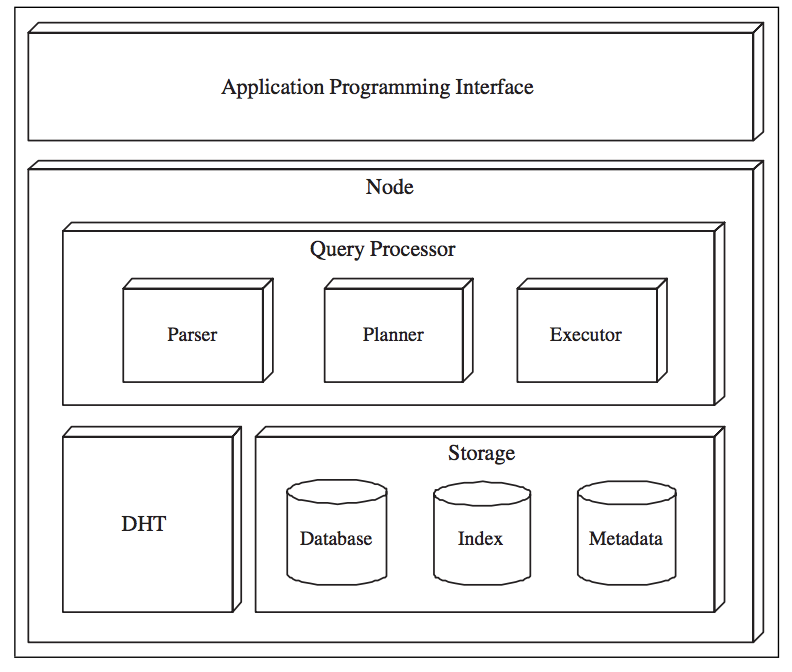
\includegraphics[width=\fscale{1}]{node_arch.png}
	\caption{A Picolo node}
	\label{fig:node_arch}
\end{figure}
The metadata depicted in the figure contains schema metadata to be exposed to the world. Nodes that wish to keep data private should not export the data's metadata to the metadata container. Suppose there is a table called \textit{users} with four columns: \textit{username}, \textit{firstname}, \textit{lastname} and \textit{email}. The exported metadata entry might look like:
\begin{center}
	\begin{tabular}{| c | c |} 
		\hline
		Entity & Keywords \\ [0.5ex] 
		\hline
		users & user, people, customer, profile\\ 
		\hline
		name & name \\
		\hline
		firstname & fn, {f\_name}, {first\_name} \\
		\hline
		lastname & ln, {l\_name}, {last\_name} \\
		\hline
		email & id, contact \\ [1ex] 
		\hline
	\end{tabular}
\end{center}
When a query is posed to any node in the system, the node first tries to fulfill it with a local query before passing it along to its neighbors. Remember, nodes in the system host data with heterogeneous schemas. Hence the keywords are used to find semantically similar data. Similarity metrics that determine whether a query matches a heterogeneous schema are not discussed here.
\newline
\newline
\textbf{Dynamic clustering}:
Semantic proximity metrics are used to find nodes that are hosting semantically similar schemas. Overtime, these nodes are discovered and are clustered together for better query performance by reducing the number of network hops required.
\newline
\newline
\textbf{Data sovereignty}: 
Picolo supports two different schema types: \textit{application controlled} and \textit{user controlled}. Applications can use user controlled schemas to put users in absolute control of data and better comply with regulations like GDPR. For example, a decentralized twitter may  want users to have control over their tweets. Users can use any third party client or Picolo's official clients to interact with their tweets effectively rendering the decentralized twitter just another client to the data albeit with better features. \newline\newline
When semantics don't allow to put user in control of data, application controlled schemas can be used. An example here would be a decentralized ticketing application where users should not be given fine grained control to selectively delete data about which tickets they bought.
\newline
\newline
\textbf{Access control}:
Applications and users may want to share data with other parties but may wish to impose access controls. There are a few ways of achieving this including building an API on top of the data or using proxy re-encryption techniques. We use a secret sharing scheme instead as it gels well with p2p nature of the system and does not introduce asymmetry like other solutions. Rules can be defined by a SQL like declarative language at any granularity desired like at the level of a single row or a cell. An example row level granularity rule looks like:\newline \newline
\texttt{SELECT  * \newline FROM users \newline WHERE email=foo@bar.com \newline NODE (SELECT nodeId FROM nodes WHERE domain=application)} \newline \newline
An example value level (only username is given access to) granularity rule looks like:\newline \newline
\texttt{ SELECT username \newline FROM users \newline WHERE email=foo@bar.com \newline NODE (SELECT nodeId FROM nodes)}
\newline
\newline
Here \texttt{NODE} is a new clause we introduce to SQL dialect.

\section{Mechanism design}
Since Picolo is an open network and nodes can't be trusted, a robust incentive and disincentive mechanism is required to realize its correct functioning. In this Section we discuss how Picolo handles failures and malicious nodes at the database and the network layers. Our mechanism design consists of these main pieces:
\begin{enumerate}
	\item Nodes need to put up a stake before they can join the network
	\item Usage of byzantine paxos
	\item Usage of trillian and writing checkpoints to a separate blockchain (ethereum most likely)
	\item Incentivizing nodes for correct behavior
\end{enumerate}
We aim to devise Casper FFG style slashing conditions based on the detection of violation of conditions of 2 and 3 above.
\newline\newline
\textbf{Assumptions in the attack model}: We assume a standard Byzantine failure model, i.e., the attacker is able to make changes to the messages at the network layer on a node or alter the behavior at the database layer for the node. The attacker is also able to coordinate the behavior of multiple nodes in real-time to achieve a desired attack scenario. We also allow for the adversary to delay communication between honest nodes so long as the adversary has the ability to do so given the topology of the overlay network (i.e. the adversary should be part of the routing path). We also assume that the attacker is computationally bound, i.e., they cannot gather enough computing resources to subvert state-of-the-art cryptographic techniques such as Elliptic curve, crypto-hash functions (such as SHA-256) or encryption schemes such as AES.
\newline\newline
\textbf{Database level Byzantine behavior}: The central tenet of our design is to use strong cryptographic primitives to push Byzantine behavior at the database layer down to either a DoS style attack vector or to the network layer where we handle it using a combination of crypto-incentives, DHT management and detection. At the database level, each node is responsible for the standard CRUD operations for a given table (or a shard). Each such operation is protected using a cryptographic signature of the entity (dapp or user) that authorizes the request. Thus a malicious node is only able to destroy the data and not alter it. For example, every write request has a signature that certifies the request. Thus, a Merkle proof audit and signature on every table can deter any malicious manipulation of the data stored. The only attack vectors that remain are various versions of DoS style disruption, where a single node or a collection of nodes disrupt the network by delaying messages or destroying the data stored. 
\newline\newline
\textbf{Network level Byzantine behavior}: Here we discuss how to handle attack vectors where the adversary can drop network messages, delete data or both. The routing layer is based on a cryptographic DHT. Thus, it is not possible for the attacker to “choose” to store a particular shard or content. The only way an attacker can do a targeted DoS is by flooding the network with a majority of nodes such that with high probability one of the compromised nodes gets the responsibility for a targeted table or shard. This mapping includes the backup nodes, thus limiting the effectiveness of a targeted attack.
\newline\newline
\textbf{Caching and replication layer incentivizes faster network links and nodes}:
The caching and replication layer prioritizes faster network links and nodes to serve requests. Thus, nodes that are dead, unresponsive or slow will get fewer requests over time. Thus, a DoS style attack scenario will cause diminishing impact over time. While the network adapts to such a disruption, it is possible for the attacker to gain enough stake and temporarily cause a slowdown. However, their stake (or trust level) would go down and they would be responsible for fewer network functions over time essentially degrading their involvement over time.	
\newline\newline
\textbf{Detection}: It is be possible to detect such DoS style behavior quickly at the network layer since the overlay topologies tend to share many links at the layer-3 on the Internet. For example, if a node appears to delay messages at the network level while maintaining fast routes and content availability might indicate malicious intent. The detection “service” can run on the nodes with the maximum stake or trust. They can detect anomalies between different layers of a potentially malicious node and agree to reduce the trust level of that node. Such a detection service can only be thwarted if the malicious node coordinates its behavior across all observable metrics such that it appears as if it is naturally faulty. For this case, it is indistinguishable from a genuinely faulty node for all practical purposes which is handled at the DHT layer (node addition, deletion, failure modes).
\newline
\newline
\textbf{Incentives}: Nodes are paid by dapp developers for storage and usage. Usage entails network ingress and egress. They also need to put up a stake in order to join the network. This stake will be slashed if they are found to be byzantine.
\newline
\newline
\textbf{Data availability proofs}: We use Proof-of-Query as a way for nodes to prove that they are storing and serving data correctly.
\newline
\newline
\textbf{Audit logs and verifiable data structures}: All data structures (primarily tables) used by Picolo are backed by an append-only log of mutations and accesses to data. Anyone can reconstruct these data structures by downloading the log and perform a full audit.

\section{MX Protocol}
This section only specifies the message exchange protocol of the system. Nodes in the network need to speak the same language for efficient discovery and communication of data (see \figref{fig:mx}). Hence the following message exchange scheme is proposed. Note that the exact mapping between the following messages and underlying transport protocol is not discussed here and may change depending on the final transport protocol chosen (QUIC vs TCP)
\newline
\newline
\textbf{PUT}:  A PUT message contains the query to be run, an optional list of nodes to run the query against and an optional max number of hops (needed in case of an empty node list). This is used for creating or updating data in the system.
\newline
\newline
\textbf{GET}: A GET message contains the query to be run, max number of hops, the number of results to retrieve, the mode of retrieval (pull vs push) and a transaction identifier. Client sends this to a server to retrieve results that match the query. Parameters in GET can be varied depending on application needs - a streaming application may choose the push mode in which server pushes data to the client as it becomes available up until the specified number is met. A latency sensitive application may choose to retrieve a small number of results in a batch in one pull.
\newline
\newline
\textbf{SEND}: Server responds to each GET message with one or more SEND messages with results. In pull mode, there is only one SEND message followed by an END message where as in push mode there are multiple SEND messages followed by an END message.
\newline
\newline
\textbf{END}: Server sends END message to indicate to the client that it has finished sending all results in response to a particular GET message.
\newline
\newline
\textbf{CLOSE}: A client can send a CLOSE message to the server to indicate that it no longer is interested in the remaining query results and close the transaction. It doesn't have to wait until all the results are retrieved.
\newline
\newline
\textbf{OK}: Server sends this message to a client as a positive acknowledgment to the client's message.
\newline
\newline
\textbf{ERROR}: Server sends this message to a client as a negatively acknowledge to the client's message.
\begin{figure}[h!] \centering
	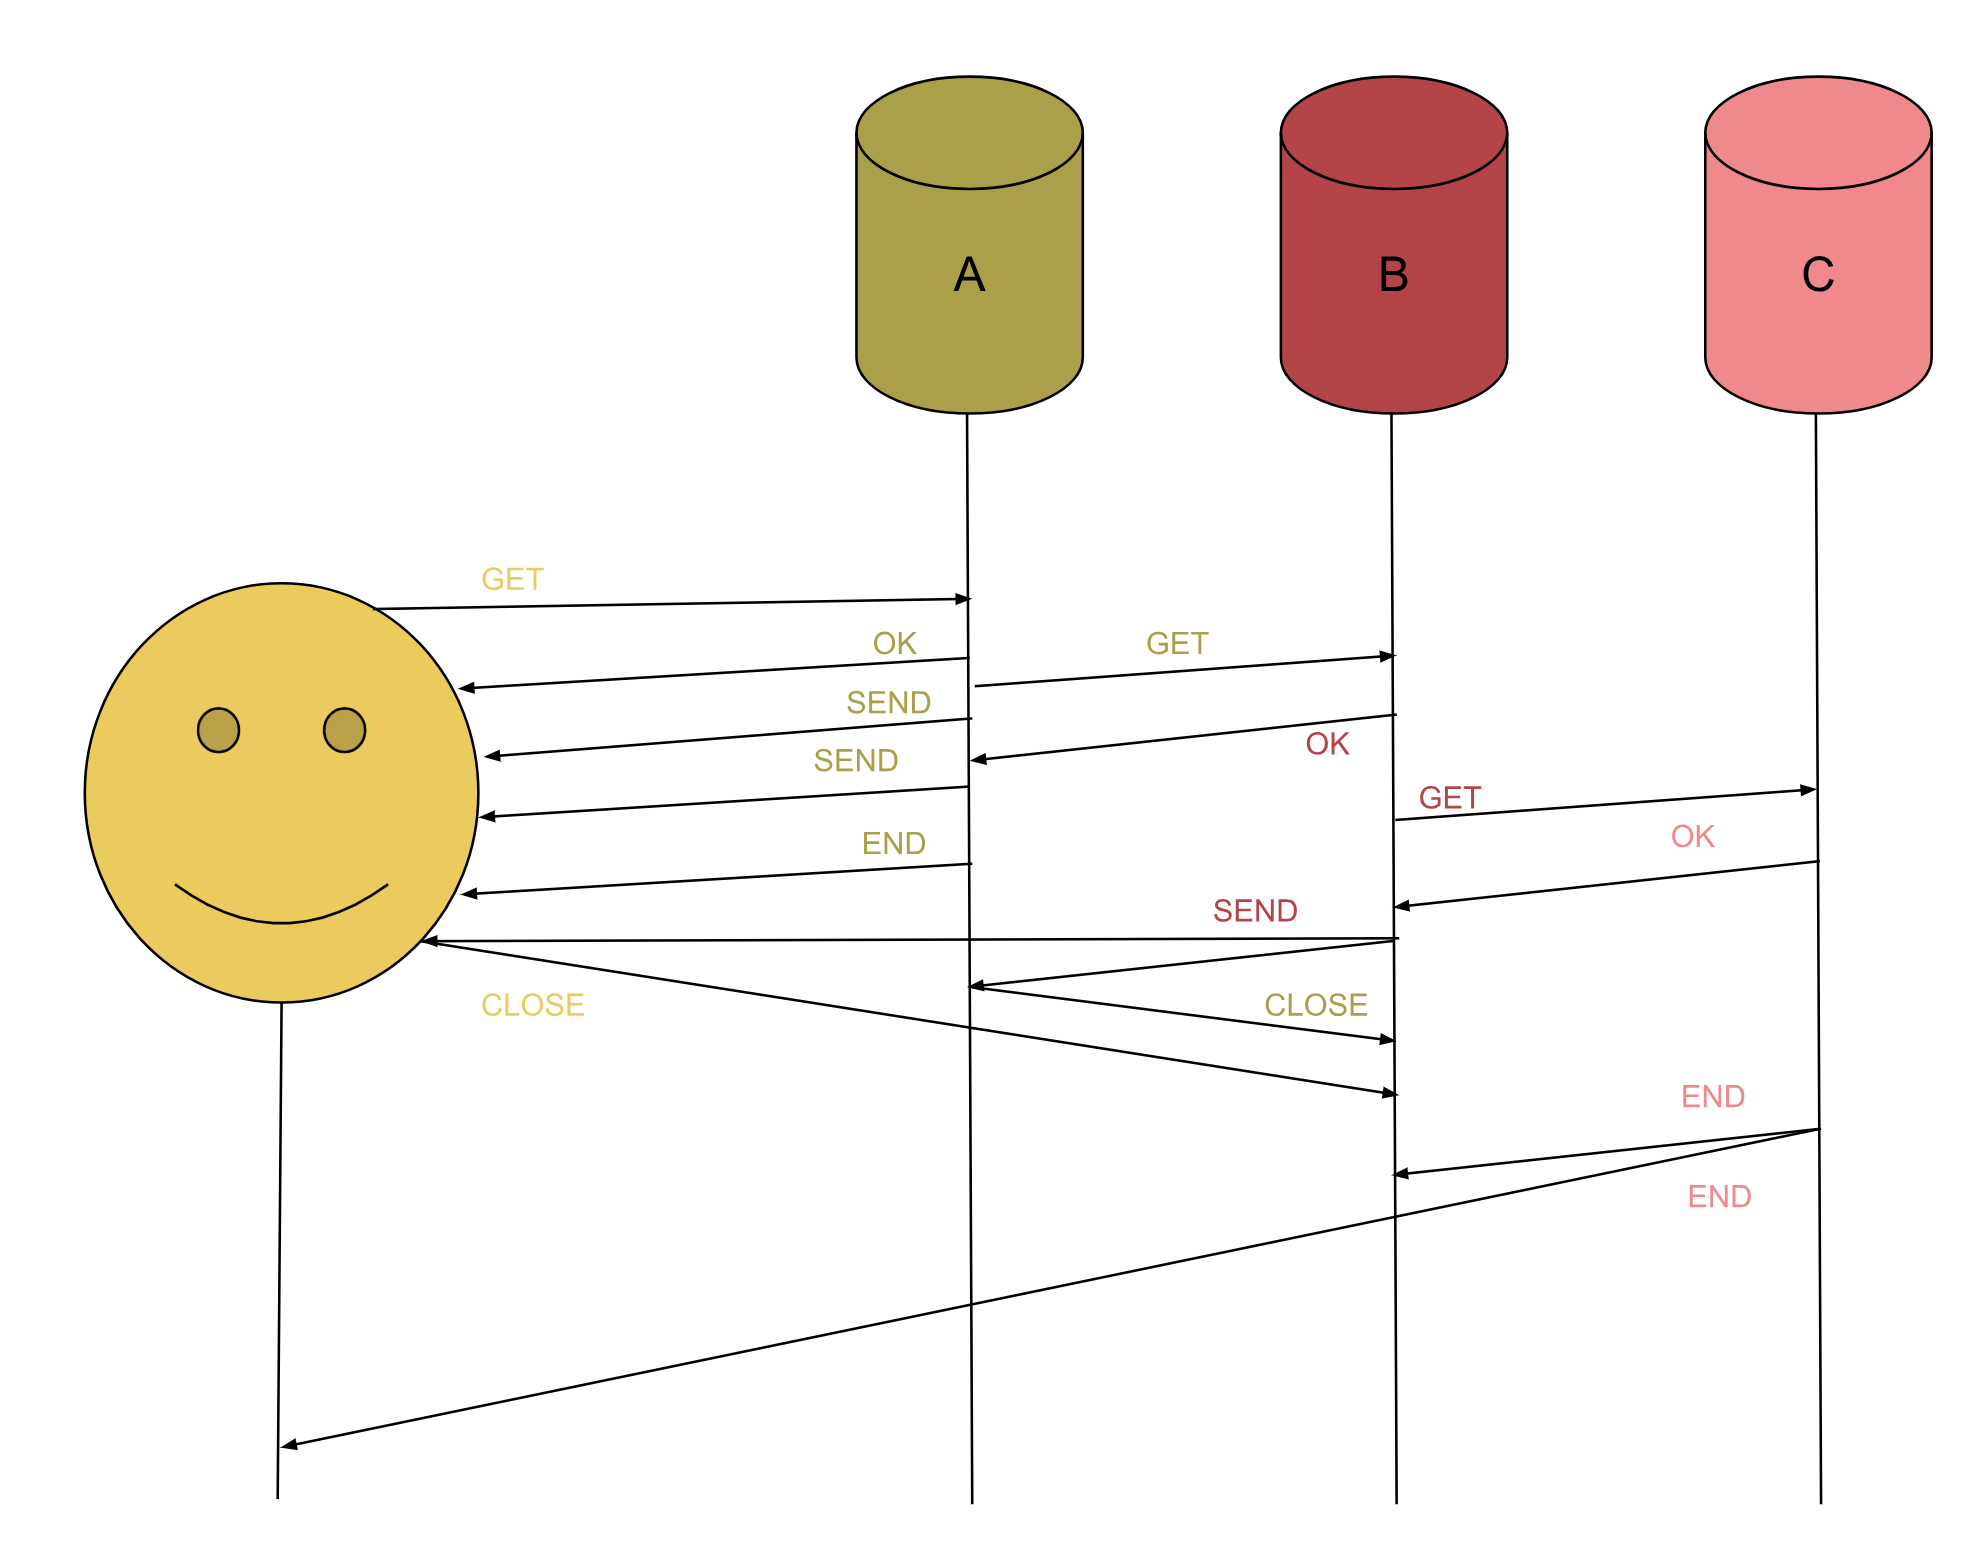
\includegraphics[width=\fscale{1}]{mx.png}
	\caption{GET message flow, time increasing from top to bottom}
	\label{fig:mx}
\end{figure}

\section{EIP and EEA}
We are contemplating an EIP (Ethereum Improvement Proposal) to give ethereum dapp developers a new choice for data storage. Not all data need to be replicated on every full node of ethereum as the need for strongest security maybe an overkill for most smart contracts. Such data can be stored on Picolo network at a contract defined replication factor. Specifically, the EIP plans to introduce SQL primitives like selections, projections, aggregates etc directly into solidity (feasibility currently being evaluated).
\newline
\newline
Picolo may also be used by ``stateless clients" to query for data that is normally hosted by ``archival nodes" in the current implementation or in the upcoming sharded implementation. Picolo's SQL capabilities make it easy for clients to construct complex queries that are not currently possible in the simple key-value lookups provided by the EVM (Ethereum Virtual Machine)
\newline\newline
Picolo fits well in the EEA (Enterprise Ethereum Alliance) stack as the solution for off-chain storage of structured data. With capabilities like access logs and fine grained access control, enterprises can confidently share data with third parties without the need for expensive and cumbersome API management solutions.

\end{document}
